\chapter{Resultados}
En este capítulo se discutirán los resultados obtenidos durante el entrenamiento de nuestra red neuronal.
Para estas pruebas usamos el conjunto de datos descrito en el capítulo. Estos resultados fueron
obtenidos usando una computadora con tarjeta gráfica NVIDIA GTX950M con
un total de 640 núcleos y una memoria de 4GB.
Estos resultados fueron obtenidos utilizando distintos esquema de redes neuronales(ver Apéndice \ref{esquemas})
\subsection{Precisión}
A continuación veremos los resultados del entrenamiento aplicados a distintas cantidades de estados ocultos $h_{t}$ .
\subsubsection{Precisión con 64 estados ocultos}

La figura \ref{RNNSIMPLE64} muestra el entrenamiento para 400 epochs de nuestra RNN simple, en esta notamos que el modelo no supera el 16\% de  precisión. Además de que oscila constantemente.

\begin{figure}[H]
	\centering
	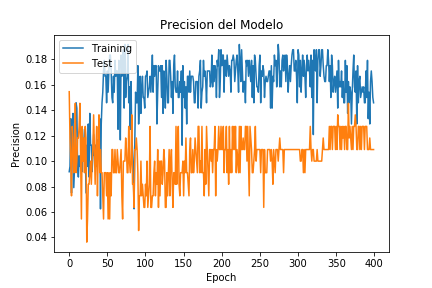
\includegraphics[width=0.7\textwidth]{Figures/rnn_64_prec}
	\caption{Precisión de RNN para 64 estados ocultos\\ Fuente: {\textit{Fuente Propia}}}
	\label{RNNSIMPLE64}
\end{figure} 
Al aplicar redes LSTM se alcanzan precisiones más altas pero a una cantidad de epochs determinada alrededor del epochs 200 la precisión del test se mantiene para una \textit{LSTM simple}.

\begin{figure}[H]
	\centering
	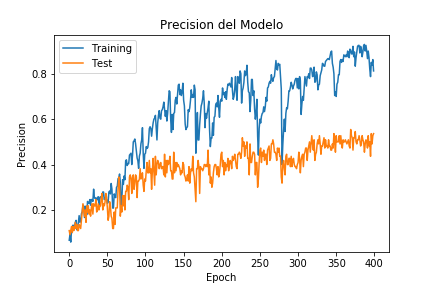
\includegraphics[width=0.7\linewidth]{Figures/lstm13_64_prec}
	\caption{Precisión de LSTM simple para 64 estados ocultos\\ Fuente: {\textit{Fuente Propia}}}
	\label{fig:lstm1364prec}
\end{figure}
\newpage
En las figuras \ref{fig:lstm6405prec} y \ref{fig:lstm6408prec} se muestran los resultados de los modelos \textit{LSTM con Dropout 0.5} y \textit{LSTM con Dropout 0.8}. En estas figuras el LSTM con Dropout 0.5 tiene una menor precisión.\\ 
\begin{figure}[H]
	\centering
	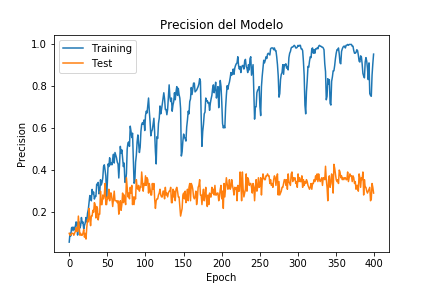
\includegraphics[width=0.7\linewidth]{Figures/lstm_64_05_prec}
	\caption{Precisión LSTM con dropout 0.5 para 64 estados ocultos\\ Fuente: {\textit{Fuente Propia}}}
	\label{fig:lstm6405prec}
\end{figure}
\begin{figure}[H]
	\centering
	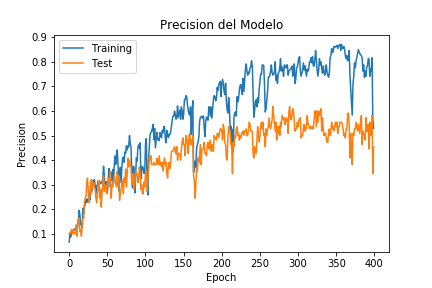
\includegraphics[width=0.7\linewidth]{Figures/lstm_64_08_prec}
	\caption{Precisión LSTM con dropout 0.8 para 64 estados ocultos\\ Fuente: {\textit{Fuente Propia}}}
	\label{fig:lstm6408prec}
\end{figure}
\newpage
El cuadro 6.1 muestra los resultados de precisión de los conjuntos test y training durante el entrenamiento luego de 300 epochs. Notamos que los mejores resultados sin llegar a overfitting son de LSTM simple y LSTM dropout (0.8).
\begin{table}[H]
	\centering
	\begin{tabular}{|c|c|c|}
		\hline
		\rowcolor{Gray}  Modelo & Precisión test(\%) & Precisión Training (\%)\\ \hline
		RNN &      10.90   &                14.58  \\ \hline
		
		LSTM &        40.00 &          73.75       \\ \hline
		
		LSTM Dropout(0.5)&  31.81    &     98.33       \\ \hline
		
		LSTM Dropout(0.8)&	0.55		&	77.91		\\ \hline
		
	\end{tabular}
	\caption{Precisión de modelos para 300 iteraciones y 64 estados ocultos}
\end{table}


\subsubsection{Precisión con 128 estados ocultos}

El RNN de la figura \ref{RNNSIMPLE}continua presentando problemas y deja de aprender para 400 epochs. Donde los resultados no varían a pesar de modificar la cantidad de estados ocultos.
\begin{figure}[H]
	\centering
	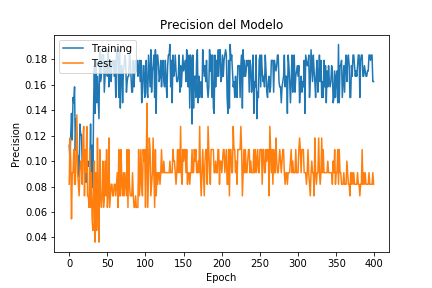
\includegraphics[width=0.7\textwidth]{Figures/rnn_prec_400_13mfcc}
	\caption{Precisión de RNN para 128 estados ocultos\\ Fuente: {\textit{Fuente Propia}}}
	\label{RNNSIMPLE}
\end{figure} 
Notamos que el LSTM simple tiende a llegar a llegar al overfitting luego de los 250 epochs.
\begin{figure}[H]
	\centering
	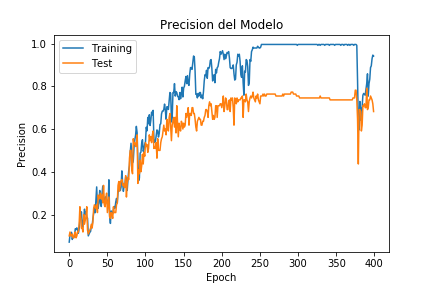
\includegraphics[width=0.7\textwidth]{Figures/lstm_400_prec_13mfcc}
	\caption{Precisión de LSTM simple para 128 estados ocultos\\ Fuente: {\textit{Fuente Propia}}}
	\label{LSTMsimpel}
\end{figure} 

Los modelos con dropout de las figuras \ref{LSTMdropout5} y 6.8 obtienen precisiones alrededor de 40\% a 60\% durante las primeras ejecuciones. 
\begin{figure}[H]
	\centering
	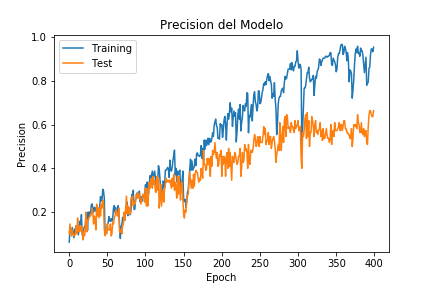
\includegraphics[width=0.7\textwidth]{Figures/lstm_400drop05_prec_13mfcc}
	\caption{Precisión de LSTM dropout 0.5 para 128 estados ocultos\\ Fuente: {\textit{Fuente Propia}}}
	\label{LSTMdropout5}
\end{figure} 


\begin{figure}[H]
	\centering
	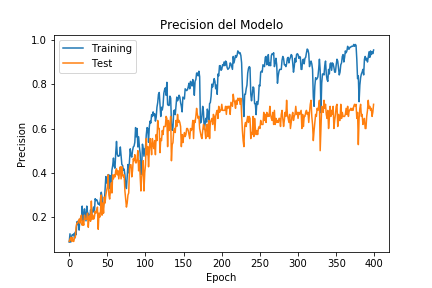
\includegraphics[width=0.7\textwidth]{Figures/lstm_400drop08_prec_13mfcc}
	\caption{Precisión de LSTM dropout 0.8 para 128 estados ocultos\\ Fuente: {\textit{Fuente Propia}}}
	\label{LSTMdropout8}
\end{figure} 
Con 128 estados ocultos el LSTM simple resulto ser un mejor modelo.\\
 El cuadro 6.2 muestra los resultados luego de 300 epochs donde los dropout obtienen mejor resultado que el LSTM y RNN, pero aún se acerca al overfitting.

\begin{table}[H]
	\centering
	\begin{tabular}{|c|c|c|}
		\hline
		\rowcolor{Gray}  Modelo & Precisión test(\%) & Precisión Training (\%)\\ \hline
		RNN &        9.09  &             17.50   \\ \hline

		LSTM &        75.45  &          99.16      \\ \hline

		LSTM Dropout(0.5) &  60.00         &     93.74         \\ \hline

		LSTM Dropout(0.8) &	67.27		&	93.74		\\ \hline

	\end{tabular}
	\caption{Precisión de modelos para 300 iteraciones y 128 estados ocultos}
\end{table}
\newpage
\subsubsection{Precisión con 256 estados ocultos}
El problema del RNN persiste en la figura \ref{fig:rnn256prec}, mientras que en la figura  \ref{fig:lstm256prec13} obtuvo resultados prometedores pero luego de los 200 epochs el conjunto training tiende a overfitting.
\begin{figure}[H]
	\centering
	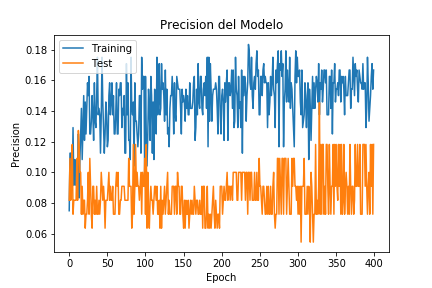
\includegraphics[width=0.7\linewidth]{Figures/rnn_256_prec}
	\caption{Precisión de RNN para 256 estados ocultos\\ Fuente: {\textit{Fuente Propia}}}
	\label{fig:rnn256prec}
	\centering
	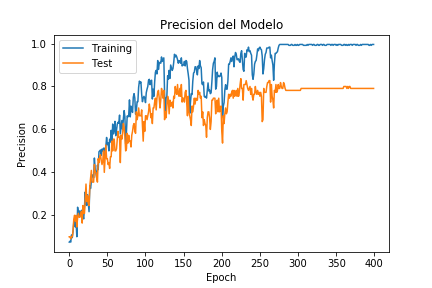
\includegraphics[width=0.7\linewidth]{Figures/lstm_256_prec13}
	\caption{Precisión LSTM simple para 256 estados ocultos\\ Fuente: {\textit{Fuente Propia}}}
	\label{fig:lstm256prec13}
\end{figure}
\newpage
 Los modelos con dropout retrasaron el overfitting, este fue más notorio a partir de los 250 epochs.
\begin{figure}[H]
	\centering
	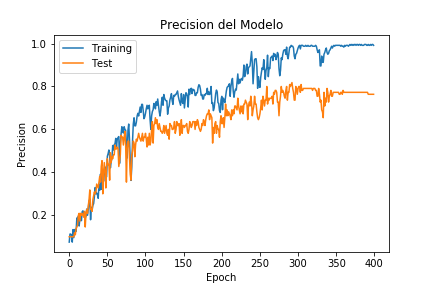
\includegraphics[width=0.7\linewidth]{Figures/lstm5_256_13prec}
	\caption{Precisión LSTM con dropout 0.5 para 256 estados ocultos\\ Fuente: {\textit{Fuente Propia}}}
	\label{fig:lstm525613prec}
	\centering
	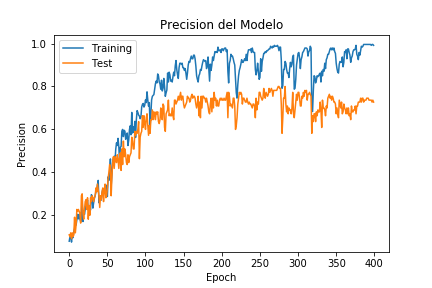
\includegraphics[width=0.7\linewidth]{Figures/lst_256_13prec}
	\caption{Precisión LSTM con dropout 0.8 para 256 estados ocultos\\ Fuente: {\textit{Fuente Propia}}}
	\label{fig:lst25613prec}
\end{figure}

El cuadro 6.3 fue tomado de las gráficas anteriores y muestra la precisión para 300 epochs.
\begin{table}[H]
	\centering
	\begin{tabular}{|c|c|c|}
		\hline
		\rowcolor{Gray}  Modelo & Precisión test(\%) & Precisión Training (\%)\\ \hline
		RNN &        9.09  &             17.50      \\ \hline
		
		LSTM &        78.18  &          99.58         \\ \hline
		
		LSTM Dropout(0.5) &  76.36         &     96.66         \\ \hline
		
		LSTM Dropout(0.8) &	82.57		&	92.91		\\ \hline
		
	\end{tabular}
	\caption{Precisión de modelos para 300 iteraciones y 256 estados ocultos}
\end{table}

%----- ERREESSSSSSSSSSSSSSSSSSSSSSSS
\subsection{Errores }
Los errores obtenidos en el entrenamiento de nuestros modelos fueron calculados usando la función de pérdida  categorical crossentropy la cual nos dirá que tan cerca nuestra predicción del valor real. En la ecuación 6.1 .
\begin{equation}
\label{CCE}
\begin{aligned}
CCE=-\frac{1}{N}\sum_{i=0}^{N}\sum_{j=0}^{J} y_{j}\log(\hat{y_{j}})+(1-y_{j})\log(1-\hat{y_{j}})
\end{aligned}
\end{equation}
\begin{itemize}
	\item N: cantidad del conjunto training.
	\item J: cantidad de clases.
	\item $\hat{y_{j}}$: valor real de la clase a predecir.
	\item $y_{j}$: predicción.
\end{itemize}





\subsubsection{Errores para 64 estados ocultos}
En las figuras \ref{fig:rnn64cost} y \ref{fig:lstm1364cost} notamos que los errores del RNN varían constantemente mientras que en LSTM estos tienden a acercarse a cero en el training, pero se mantienen en margenes alto para el test.
\begin{figure}[H]
	\centering
	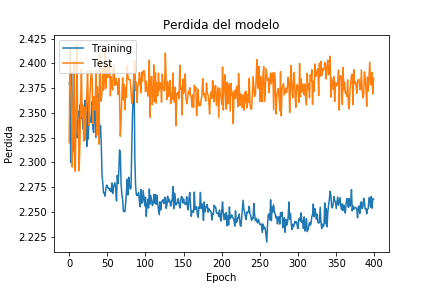
\includegraphics[width=0.7\linewidth]{Figures/rnn_64_cost}
	\caption{Perdida LSTM para 64 estados ocultos\\ Fuente: {\textit{Fuente Propia}}}
	\label{fig:rnn64cost}
	
	\centering
	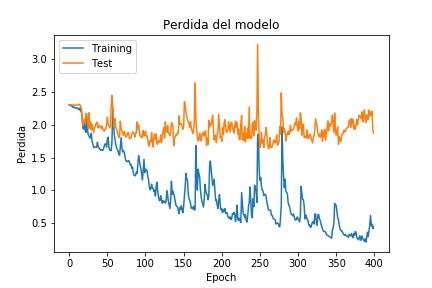
\includegraphics[width=0.7\linewidth]{Figures/lstm13_64_cost}
	\caption{Perdida LSTM  para 64 estados ocultos \\ Fuente: {\textit{Fuente Propia}}}
	\label{fig:lstm1364cost}
\end{figure}
\newpage
Para la aplicación de LSTM con Dropout, los resultados fueron menos estables para LSTM con Dropout 0.5. Mientras obtuvo mejores resultados para LSTM con dropout 0.8 .
\begin{figure}[H]
	\centering
	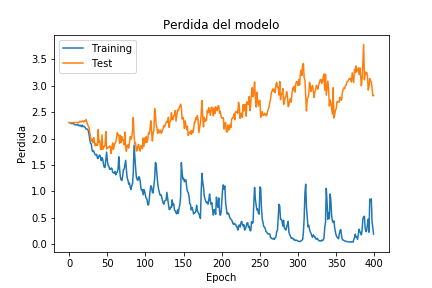
\includegraphics[width=0.7\linewidth]{Figures/lstm_64_05_cost}
	\caption{Perdida LSTM con dropout 0.5 para 64 estados ocultos\\ Fuente: {\textit{Fuente Propia}}}
	\label{fig:lstm6405cost}
	\centering
	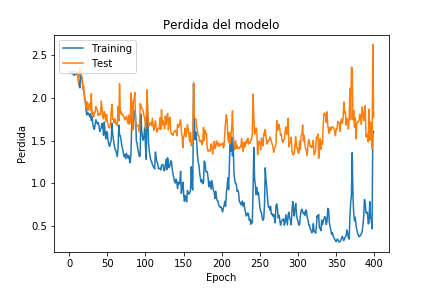
\includegraphics[width=0.7\linewidth]{Figures/lstm_64_08_cost}
	\caption{Perdida LSTM con dropout 0.8 para 64 estados ocultos\\ Fuente: {\textit{Fuente Propia}}}
	\label{fig:lstm6408cost}
\end{figure}

 En el cuadro 6.4 mostramos los errores para 300 epochs en los modelos RNN y LSTM Dropout 0.5 tuvieron los errores más altos.	Mientras que los modelos más estables fueron LSTM y LSTM con Dropout 0.8. 
\begin{table}[H]
	\centering
	\begin{tabular}{|c|c|c|}
		\hline
		\rowcolor{Gray}  Modelo & Error test& Error Training \\ \hline
		RNN &        2.378  &             2.235       \\ \hline
		LSTM &        1.960 &          0.598     \\ \hline
		LSTM Dropout(0.5) &  3.074         &    0.073        \\ \hline
		LSTM Dropout(0.8) &	1.419		&	0.581	\\ \hline
	\end{tabular}
	\caption{Errores de los conjuntos test y training para 300 iteraciones y 64 estados ocultos}
\end{table}

\subsubsection{Errores para 128 estados ocultos}
Los modelos RNN muestras muestran errores muy altos. Observamos en la figura \ref{LSTMsimplecost} que los errores de la LSTM simple tienden a cero a partir de 250 epochs.
\begin{figure}[H]
	\centering
	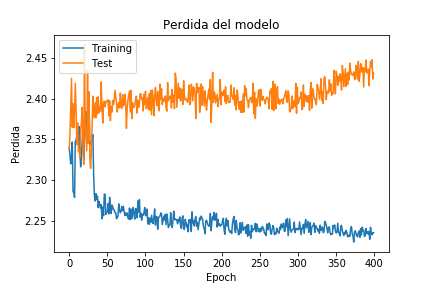
\includegraphics[width=0.7\textwidth]{Figures/rnn_cost_400_13mfcc}
	\caption{Perdida de RNN para 128 estados ocultos\\ Fuente: {\textit{Fuente Propia}}}
	\label{RNNSIMPLEcost}
\end{figure} 


\begin{figure}[H]
	\centering
	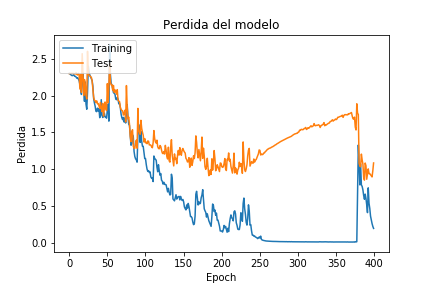
\includegraphics[width=0.7\textwidth]{Figures/lstm_400_cost_13mfcc}
	\caption{Perdida de LSTM para 128 estados ocultos\\ Fuente: {\textit{Fuente Propia}}}
	\label{LSTMsimplecost}
\end{figure} 
Las figuras \ref{LSTMdropout5cost} y \ref{LSTMdropout8cost} son obtienen errores entre 0 y 3. A medida que aumenta el epochs nuestro error en el conjunto test empieza a incrementarse.
\begin{figure}[H]
	\centering
	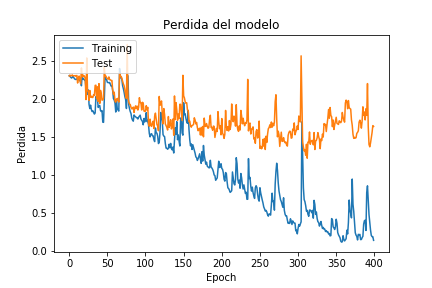
\includegraphics[width=0.7\textwidth]{Figures/lstm_400drop05_cost_13mfcc}
	\caption{Perdida de LSTM dropout 0.5 para 128 estados ocultos\\ Fuente: {\textit{Fuente Propia}}}
	\label{LSTMdropout5cost}
\end{figure} 


\begin{figure}[H]
	\centering
	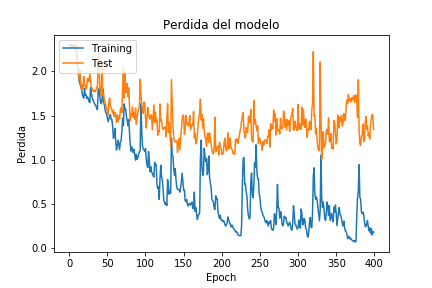
\includegraphics[width=0.7\textwidth]{Figures/lstm_400drop08_cost_13mfcc}
	\caption{Perdida de LSTM dropout 0.8 para 128 estados ocultos\\ Fuente: {\textit{Fuente Propia}}}
	\label{LSTMdropout8cost}
\end{figure} 

En cuadro 6.5 mostramos los errores luego de 300 iteraciones donde observamos que los modelos LSTM y dropout 0.8 tienen menores errores durante la predicción usando el conjunto test.

\begin{table}[H]
	\centering
	\begin{tabular}{|c|c|c|}
		\hline
		\rowcolor{Gray}  Modelo & Error test& Error Training \\ \hline
		RNN &        2.414  &             2.240      \\ \hline
		LSTM &        1.489  &          0.011       \\ \hline
		LSTM Dropout(0.5) & 1.647         &     0.230          \\ \hline
		LSTM Dropout(0.8) &	1.329		&	0.2150	\\ \hline
	\end{tabular}
	
	\caption{Errores de los conjuntos test y training para 400 iteraciones y 128 estados ocultos}
\end{table}
\newpage
\subsubsection{Errores para 256 estados ocultos}
Al aumentar la cantidad de estados ocultos se noto un decrecimiento rápido del error en el LSTM en comparación al RNN que no ha sido afectado por los cambios de estados ocultos.
\begin{figure}[H]
	\centering
	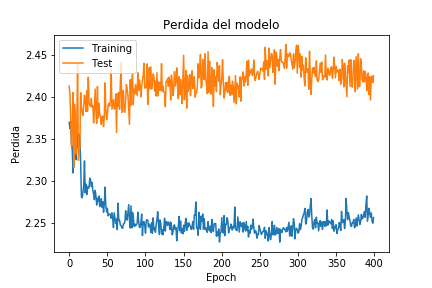
\includegraphics[width=0.7\linewidth]{Figures/rnn_256_cost}
	\caption{Perdida de RNN para 256 estados ocultos\\ Fuente: {\textit{Fuente Propia}}}
	\label{fig:rnn256cost}
	
	\centering
	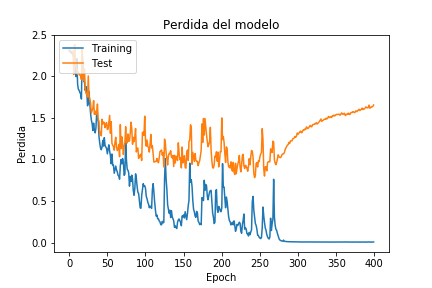
\includegraphics[width=0.7\linewidth]{Figures/lstm_256_cost13}
	\caption{Perdida de LSTM para 256 estados ocultos\\ Fuente: {\textit{Fuente Propia}}}
	\label{fig:lstm256cost13}
\end{figure}
\newpage
Los modelos LSTM con dropout tienen errores entre 1.5 y 0.2 rápidamente pero luego estos aumentan a medida que se incrementa el epochs.
\begin{figure}[H]
	\centering
	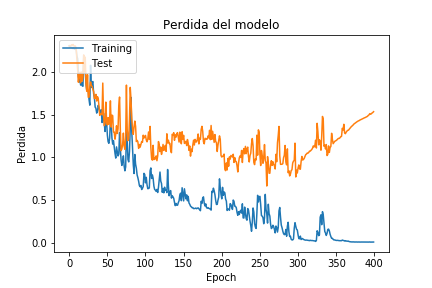
\includegraphics[width=0.7\linewidth]{Figures/lstm5_256_13cost}
	\caption{Perdida de LSTM con Dropout 0.5 para 256 estados ocultos\\ Fuente: {\textit{Fuente Propia}}}
	\label{fig:lstm525613cost}
	
	\centering
	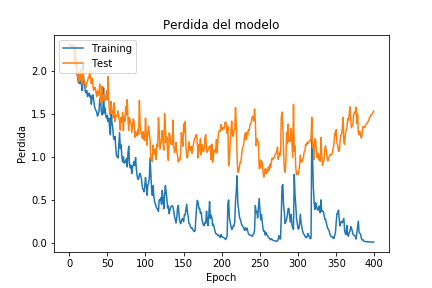
\includegraphics[width=0.7\linewidth]{Figures/lstm_256_13cost}
	\caption{Perdida de LSTM con Dropout 0.8 para 256 estados ocultos\\ Fuente: {\textit{Fuente Propia}}}
	\label{fig:lstm25613cost}
\end{figure}
El cuadro 6.6 muestra los resultados para 300 epochs, en esta cantidad de iteraciones nuestros modelos con Dropout tienen resultados cercanos a 0 pero gráficamente (ver figuras \ref{fig:lstm525613cost} y \ref{fig:lstm25613cost}) los errores aumentan luego de 300 epochs.


\begin{table}[H]
	\centering
	\begin{tabular}{|c|c|c|}
		\hline
		\rowcolor{Gray}  Modelo & Error test& Error Training \\ \hline
		RNN &        2.427 &             2.242     \\ \hline
		LSTM &        1.3170  &          0.008    \\ \hline
		LSTM Dropout(0.5) &  0.815       &     0.148        \\ \hline
		LSTM Dropout(0.8) &	0.825		&	0.224	\\ \hline
	\end{tabular}
	\caption{Errores de los conjuntos test y training para 300 iteraciones y 256 estados ocultos}
\end{table}

\subsection{Modelo para reconocimiento de voz}
A continuación se presentan los resultados obtenidos por el modelo de 2 capas LSTM y 2 dropout(ver esquema \ref{2LSTMESQUEMA})
\subsubsection{Precisión}
La figura \ref{fig:modelprec} nos muestra la precisión de nuestro modelo. Este es más controlado debido a los 2 dropout que evitan el overfitting. Este modelo fue testeado usando 64 y 128 estados ocultos.

\begin{figure}[H]
	\centering
	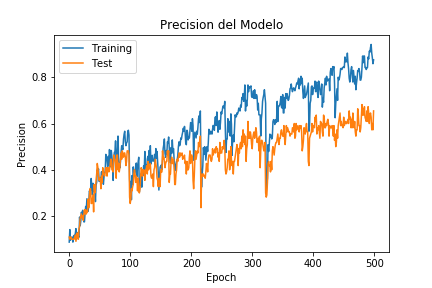
\includegraphics[width=0.7\linewidth]{Figures/MODEL_prec}
	\caption{Precisón de modelo con 2 LSTM y 2 - 64 estados ocultos}
	\label{fig:modelprec}
\end{figure}	

\begin{figure}
	\centering
	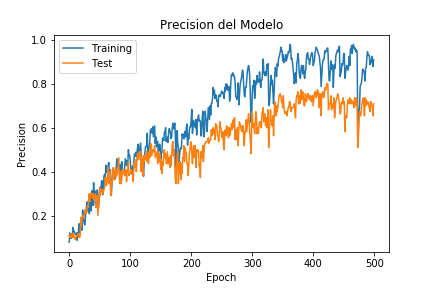
\includegraphics[width=0.7\linewidth]{Figures/prec500}
	\caption{Precisón de modelo con 2 LSTM y 2 - 128 estados ocultos }
	\label{fig:prec500}
\end{figure}

En el cuadro 6.7 observamos que obtuvimos una precisión de 65.45\% usando 64 estados ocultos y una precisión de 70.91\% usando 128 estados ocultos.
\begin{table}[H]
	\centering
	\begin{tabular}{|c|c|c|}
		\hline
		\rowcolor{Gray}  Modelo 2LSTM 2 Dropout & Precisión test(\%) & Precisión Training (\%)\\ \hline
		64 estados ocultos&     65.45    &                87.50  \\ \hline
		128 estados ocultos&	70.91		&					90.83	\\ \hline
	\end{tabular}
	\caption{Precisión de modelos para 500 iteraciones }
\end{table}

\subsubsection{Errores del modelo}
Las figuras \ref{fig:modelcost}  y \ref{fig:modelcost} muestran los errores para 64 y 128 estados ocultos. Donde observamos que para 64 el error del test no excede el valor de 2 y tiene cierta estabilidad. Por el contrario el modelo con 128 estados ocultos continua oscilando más.
\begin{figure}
	\centering
	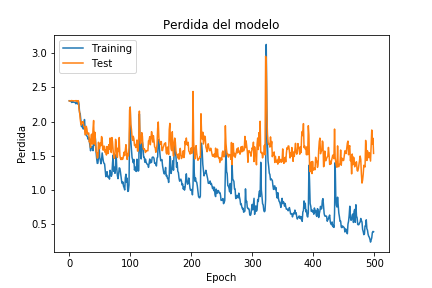
\includegraphics[width=0.7\linewidth]{Figures/MODEL_cost}
	\caption{Error del modelo con 2 LSTM y 2 - 64 estados ocultos\\ Fuente: {\textit{Fuente Propia}}}
	\label{fig:modelcost}

	\centering
	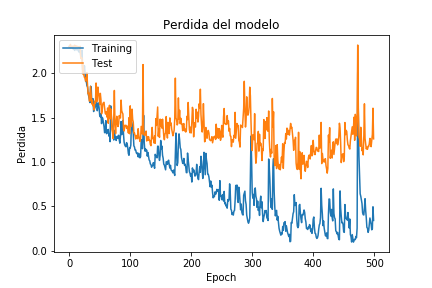
\includegraphics[width=0.7\linewidth]{Figures/cost500}
	\caption{Error del modelo con 2 LSTM y 2 - 128 estados ocultos\\ Fuente: {\textit{Fuente Propia}}}
	\label{fig:cost500}
\end{figure}
\newpage

El cuadro 6.8 nos muestra el error final luego de 500 iteraciones para nuestros modelos con 64 y 128 estados ocultos. Donde este último obtuvo mejores resultados finales.
\begin{table}[H]
	\centering
	\begin{tabular}{|c|c|c|}
		\hline
		\rowcolor{Gray}  Modelo 2LSTM 2 Dropout & Error test& Error Training \\ \hline
		64 estados ocultos &        1.5330 &             0.3858     \\ \hline
		128 estados ocultos	&		1.2617 	&				0.3413   \\ \hline
	\end{tabular}
	\caption{Errores de los conjuntos test y training para 500 iteraciones}
\end{table}